\subsection{Analisis ROC}

Grafik \textit{Receiver Operating Characteristics} (ROC) adalah teknik untuk
memvisualisasi, mengelompokan, dan memilih pengklasifikasi berdasarkan
performansinya.

\subsubsection{Performansi pengklasifikasi}

Misalkan pada permasalahan pengklasifikasian menggunakan hanya dua kelas.
Setiap instan \textit{I} dipetakan pada sebuah elemen set $ {p, n} $ yaitu
kelas positif dan negatif.
Model klasifikasi (atau pengklasifikasi) adalah pemetaan dari instan terhadap
kelas yang diprediksi.
Beberapa model klasifikasi menghasilkan keluaran \textit{continuous} yang mana
\textit{threshold} tertentu digunakan untuk memprediksi target kelas.
Model lain menghasilkan label kelas diskrit mengindikasikan hanya prediksi
kelas dari instan.
Untuk membedakan antara kelas sebenarnya dengan kelas prediksi digunakan label
$ { Y, N } $ untuk prediksi kelas yang dihasilkan oleh model.

Diberikan sebuah pengklasifikasi dan sebuah instan, ada empat kemungkinan
keluaran.
Jika kelas instan adalah positif dan diklasifikasi positif, maka dihitung
sebagai \textit{true positive}, jika diklasifikasi negatif, maka dihitung
sebagai \textit{false negative}.
Jika instan negatif dan diklasifikasi sebagai negatif, maka dihitung sebagai
\textit{true negative}, jika diklasifikasi positif, maka dihitung sebagai
\textit{false positive}.
Jika diberikan sebuah pengklasifikasi dan sebuah set instan (set pengujian),
maka dapat dibuat matriks \textit{confusion} (disebut juga tabel
\textit{contingency}) yang merepresentasikan disposisi dari kumpulan instan,
seperti pada Gambar \ref{fig:confusion_matrix}.

\begin{figure}[b!]
	\centering
	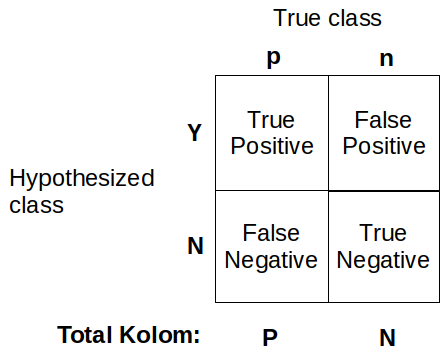
\includegraphics[keepaspectratio=true,scale=0.5]{confusion_matrix}
	\caption{Matriks \textit{confusion}}
	\label{fig:confusion_matrix}
\end{figure}

Laju \textit{true positive} (disebut juga dengan \textit{hit rate} dan
\textit{recall}) dari sebuah pengklasifikasi dapat dihitung dengan,

\begin{align*}
	\textit{tp rate} &\approx
			\frac{\text{Jumlah klasifikasi positif}}
				{\text{Total positif}} \\
		&= \frac{TP}{P}
\end{align*}
Laju \textit{false positive} (disebut juga \textit{false alarm rate}) dari
pengklasifikasi adalah
\begin{align*}
	\textit{fp rate} &\approx \frac{\text{Jumlah klasifikasi negatif}}
			{\text{Total negatif}} \\
		&= \frac{FP}{N}
\end{align*}
Istilah lainnya yang berkaitan dengan kurva ROC adalah,
\[
	\text{precision} = \frac{TP}{TP + FP}
\]
\[
	\text{accuracy} = \frac{TP + TN}{P + N}
\]
\[
	\text{sensitivity} = \text{recall}
\]
\begin{align*}
	\text{specificity}
		&= \frac{\text{Jumlah true negative}}
			{\text{jumlah false positive}
			+ \text{jumlah true negative}} \\
		&= 1 - \textit{fp rate}
\end{align*}
\[
	\text{positive predictive value} = \text{precision}
\]

\subsubsection{Ruang ROC}

Grafik ROC adalah grafik dua dimensi yang mana \textit{tp rate} diplot pada
$ Y $ dan \textit{fp rate} diplot pada sumbu $ X $.
Sebuah grafik ROC menggambarkan lawan antara keuntungan (true positive) dan
biaya (false positive).
Gambar \ref{fig:roc_graph} memperlihatkan grafik ROC dengan lima klasifikasi
dari A sampai E.

\begin{figure}[t!]
	\centering
	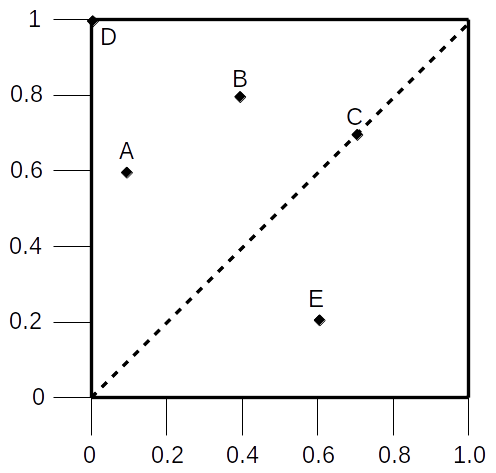
\includegraphics[keepaspectratio=true,scale=0.5]{roc_graph}
	\caption{Grafik ROC dengan lima klasifikasi}
	\label{fig:roc_graph}
\end{figure}

Klasifikasi diskrit yaitu yang mengeluarkan hanya sebuah label kelas.
Setiap pengklasifikasi diskrit menghasilkan sebuah pasangan
(\textit{fp rate}, \textit{tp rate}) yang berkorespondensi dengan satu titik di
ruang ROC.

Titik (0,0) merepresentasikan klasifikasi yang tidak pernah positif dan tidak
pula negatif. Sebaliknya, titik (1,1) merepresentasikan klasifikasi positif.
Titik (0,1) merepresentasikan klasifikasi sempurna, contohnya D.

Titik dalam ruang ROC lebih baik daripada yang lainnya bila berada di bagian
kiri atas (\textit{tp rate} tinggi, \textit{fp rate} rendah, atau keduanya).
Pengklasifikasi yang berada di sisi kiri dari grafik ROC, dekat sumbu $X$, bisa
disebut "konservatif": menghasilkan klasifikasi positif hanya dengan bukti yang
kuat sehingga menghasilkan beberapa galat positif, tapi seringkali memiliki
\textit{tp rate} yang rendah.
Pengklasifikasi di bagian kanan-atas dari grafik ROC bisa disebut "liberal":
menghasilkan klasifikasi positif dengan bukti yang lemah atau menghasilkan
hampir semuanya positif secara tepat, tapi memiliki \textit{fp rate} yang
tinggi.
Pada gambar \ref{fig:roc_graph}, pengklasifikasi $A$ lebih konservatif daripada
$B$.

\subsubsection{Performansi acak}

Garis diagonal $ y = x $ merepresentasikan strategi yang secara acak memilih
kelas.
Sebagai contohnya, jika sebuah pengklasifikasi secara acak memilih kelas
positif, maka didapat setengahnya positif dan setengahnya negatif menghasilkan
titik (0.5,0.5) di ruang ROC.
Jika secara acak mendapatkan 90\% positif, maka \textit{fp rate}-nya juga akan
meningkat menjadi 90\%, menghasilkan titik (0.9,0.9) di ruang ROC.
Pada gambar \ref{fig:roc_graph} klasifikasi C bisa dibilang secara acak menebak
kelas positif 70\%.

Pengklasifikasi yang berada di bawah kanan diagonal bekerja lebih buruk dari
pengklasifikasi yang menerka secara acak.
Bagian ini biasanya kosong dalam grafik ROC.

\subsubsection{Kurva \textit{Area Under ROC}}

Sebuah kurva ROC adalah gambar dua dimensi dari performansi pengklasifikasi.
Untuk membandingkan pengklasifikasi bisa dengan menurunkan performansi ROC
menjadi nilai skalar tunggal merepresentasikan performansi yang diharapkan.
Metode yang paling umum yaitu menghitung wilayah di bawah kurva ROC, disingkat
dengan AUC (\textit{Area Under an ROC}).
Secara AUC adalah bagian dari area dari sebuah bujur sangkar, nilainya akan
selalu antara 0 dan 1.0.
Karena perkiraan secara acak menghasilkan garis diagonal antara (0,0) dan
(1,1), yang memiliki wilayah 0.5, maka tidak ada pengklasifikasi yang 
seharusnya memiliki AUC kurang dari 0.5.
